\section{Definisi \textit{Micro Frameworki}}

\textit{Microframework} adalah istilah yang digunakan untuk merujuk pada kerangka kerja web minimalis. Kerangka ini sangat berbeda dengan kerangka kerja tumpukan penuh. Juga tidak memiliki sebagaian besar fungsionalitas yang umum yang ada dalam kerangka kerja aplikasi web lengkap, seperti:
\begin{enumerate}
\item Akun, otentikasi, otorisasi, peran, dll.
\item Abtraksi basis data melalui pemetaan objek-relasional.
\item Validai  \textit{input} dan sanitasi \textit{input}.
\item Mesin \textit{template web}.
\end{enumerate}

Biasanya, sebuah \textit{microframework} memfasilitasi menerima permintaan HTTP, merutekan permintaan HTTP ke \textit{controller} yang sesuai, mengirim \textit{controller}, dan mengembalikan respons HTTP. \textit{Microframeworks} seringkali dirancang khusus untuk membangun API untuk layanan atau aplikasi lain. Misalnya, Lumen \textit{microframework} dirancang untuk pengembangan \textit{Microservices} dan pengembangan API. \textit{Microframework}, sebuah \textit{tool} yang digunakan untuk \textit{project} yang lebih kecil dan penggunaan untuk kasus yang spesifik. Ini sama saja dengan menyederhanakan \textit{framework} agar lebih mudah dalam implementasi dan menyediakan \textit{testing} dan \textit{deployment} yang lebih cepat. \textit{Microframework} mengeluarkan banyak sekali komponen yang ada pada pengaturanan \textit{full-stack}, termasuk:
\begin{enumerate}
\item \textit{Web template engine}
\item \textit{Input validation}
\item \textit{Database abstraction}
\item \textit{Roles, accounts, and authentication}
\end{enumerate}

Kerugian menggunakan  \textit{microframework} adalah saat  \textit{project} mulai tumbuh besar dengan cepat. Dimana  \textit{microframework} tidak memiliki fitur yang dibutuhkan untuk mengakomodasi pertumbuhan  \textit{website}. Dengan kata lain kamu kehilangan fleksibelitas.  \textit{Micro-framework} lebih baik saat digunakan untuk  \textit{project} kecil yang membutuhkan kesederhanaan,  \textit{overhead} yang rendah dan  \textit{deployment} yang cepat.  \textit{Developer} yang sudah berpengalaman bisa saja menggunakan  \textit{microframework} pada awal  \textit{project} dan menambahkan tambahan  \textit{microframework} jika diperlukan. Hal ini merupakan pilihan yang menarik, tetapi untuk pemula dan  \textit{developer} menengah harus menghindari ini \cite{fadhilnet}.

\section{Jenis-Jenis \textit{Framework} Python serta Kelebihan dan Kekurangan}

\subsection{Django}

Django adalah kerangka kerja web Python yang memungkinkan individu dalam pengembangan yang bersih dan cepat. Kerangka kerja web secara umum dikatakan sebagai campuran komponen yang membantu pengembang mengembangkan situs web lebih cepat dan mudah. Karena itu, ini adalah kerangka kerja sumber bebas dan terbuka. Ini dapat disebut sebagai kerangka kerja yang memungkinkan pengembang untuk mengambil konsep penyelesaian secepat mungkin. Django sebagai kerangka kerja membantu mengurangi beberapa kesalahan keamanan umum yang dapat diawasi dengan mudah saat mengembangkan aplikasi. Skalabilitas adalah fitur lain yang disediakan oleh kerangka ini.

Django memiliki \textit{tagline "The web framework for perfectionists with deadlines"}, bagaimana tidak, karena secara \textit{default} Django sudah memiliki berbagai modul umum yang biasa digunakan ketika mengembangkan aplikasi web.

Kelebihan:
\begin{enumerate}
\item Cepat.

Ini telah dirancang sedemikian rupa untuk membantu pengembang membuat aplikasi secepat mungkin. Dari ide, produksi hingga rilis, Django membantu menjadikannya efektif dan efisien. Dengan demikian itu menjadi solusi ideal bagi pengembang yang memiliki fokus utama pada tenggat waktu.

\item Penuh dimuat.

Ini bekerja dengan cara yang mencakup puluhan tambahan untuk membantu dengan otentikasi pengguna, peta situs, administrasi konten, umpan RSS, dan banyak lagi hal-hal seperti itu. Aspek-aspek ini membantu dalam melaksanakan proses pengembangan web sepenuhnya.

\item Aman.

Ketika melakukannya di Django, dipastikan bahwa pengembang tidak melakukan kesalahan yang terkait dengan keamanan. Beberapa kesalahan umum termasuk injeksi SQL, pemalsuan permintaan lintas situs, clickjacking dan skrip lintas situs. Untuk mengelola nama pengguna dan kata sandi secara efektif, sistem otentikasi pengguna adalah kuncinya.

\item Dapat diukur.

Untuk memenuhi permintaan lalu lintas terberat, manfaat kerangka Django dapat dilihat. Oleh karena itu, situs tersibuk menggunakan media ini untuk dengan cepat memenuhi permintaan lalu lintas.

\item Serbaguna.

Manajemen konten,\textit{ platform} komputasi ilmiah, dan bahkan organisasi besar, semua aspek ini dikelola secara efisien dengan penggunaan Django.

\item Dokumentasi yang sangat lengkap dan kamu tidak perlu banyak - banyak \textit{googling} karena sudah disediakan contoh.
\item Modul administrasi yang \textit{auto generate} sesuai dengan model yang didefinisikan di dalam aplikasi. Lebih dari sekedar \textit{CRUD generator}.
\item Sistem migrasi \textit{database} otomatis yang tidak perlu kamu tulis \textit{script}-nya. Cukup mengubah class dan struktur \textit{database} pun berubah sesuai perubahan terakhir.
\item Memiliki sistem form yang kokoh.
\item Sudah \textit{built-in} untuk sistem autentikasi dan roles bila Anda menggunakan \textit{relational database} yang didukung Django seperti MySQL dan PostgreSQL.
\item Memiliki ekstensi - ekstensi yang bisa membuat kamu lebih produktif seperti \textit{Django Rest Framework, Django Rest Auth, Django Celery, Django Mongoengine, GeoDjango,} dan lainnya.
\item Memiliki \textit{template engine} sendiri yang lebih \textit{powerful}.
\item Kompatibilitas dengan berbagai modul dan \textit{library} lain.
\end{enumerate}

Kekurangan:
\begin{enumerate}
\item Menggunakan pola perutean, tentukan URL-nya
\item Django terlalu monolitik
\item Semuanya didasarkan pada Django ORM
\item Komponen dikerahkan bersama
\item Pengetahuan tentang sistem lengkap diperlukan untuk bekerja.
\end{enumerate}

\subsection{Flask}

Python adalah Flask, yang merupakan kerangka kerja mikro untuk Python berdasarkan teknologi seperti Werkzeug, Jinja 2. Flask pada dasarnya adalah kerangka kerja web Python yang dibangun dengan inti kecil dan selanjutnya mudah untuk memperpanjang ekstensi Flask lebih berorientasi Python daripada Django karena beberapa alasan yang jelas. Karena ada sedikit kode \textit{boilerplate} yang harus ditangani oleh pengembang, Flask adalah kerangka kerja web yang mungkin tidak perlu dikerjakan pengembang lebih lama untuk memahami mereka. Banyak aplikasi terkenal di luar sana ditulis dalam kerangka kerja Flask seperti Pinterest, LinkedIn dan halaman web komunitas untuk Flask itu sendiri \cite{ramdani2018clustering}.

Flask sendiri dapat dikatakan sebagai \textit{web framework} yang fleksibel terhadap library apapun untuk Python. Selain itu dokumentasinya yang jelas membuat Flask sangat diminati oleh kawula muda.

Kelebihan:
\begin{enumerate}
	\item \textit{Framework} yang mudah untuk digunakan dan dipahami.
	\item Berisi pengembangan server dan \textit{debugger}.
	\item \textit{RESTfull request dispatching}.
	\item Menggunakan Jinja2 \textit{template engine}.
	\item Dukungan untuk \textit{secure cookies} pada sisi \textit{client}.
	\item 100\% \textit{Web Server Gateway Interface} (WSGI).
	\item Berbasis \textit{Unicode} yaitu suatu standar yang dirancang untuk mengizinkan \textit{text} dan \textit{symbol} dari semua tulisan untuk menampilkan dan dimanipulasi secara konsisten oleh komputer.
	\item Dokumentasi yang ekstensif.
	\item Kompatibilitas \textit{Google App Engine}.
\end{enumerate}

Kekurangan:
\begin{enumerate}
\item Fungsionalitas
\end{enumerate}

Beberapa fitur Flask yang perlu kamu ketahui antara lain:
\begin{enumerate}
	\item \textit{Built-in development server} dan \textit{debugger}.
	\item Terintegrasi dengan unit \textit{testing}.
	\item RESTful.
	\item Menggunakan \textit{template engine} Jinja2.
	\item Mendukung \textit{secure cookie}.
	\item 100\% mendukung WSGI 1.0.
	\item \textit{Unicode based}.
	\item Dokumentasi yang baik.
	\item Komunitas yang kuat.
\end{enumerate}

\subsection{Tornado}

Tornado adalah salah satu kerangka kerja web terbaik dari bahasa pemrograman Python. Kerangka kerja ini memungkinkan pendekatan yang lebih bersih untuk pemrograman server Web dan memiliki fokus yang tajam pada operasi non-pemblokiran, dapat meningkatkan skala ke sejumlah besar koneksi terbuka \cite{panjaitan2018sistem}.

Kelebihan:
\begin{enumerate}
\item Dukungan bawaan

Tornado hadir dengan dukungan bawaan dan menemukan solusi untuk sebagian besar aspek pengembangan Web yang membosankan seperti templat, pelokalan, cookie yang ditandatangani, dll. Tornado juga memungkinkan pengguna untuk mencampurnya dengan kerangka kerja lain, dengan cuplikan yang sesuai, sesuai untuk kebutuhan mereka.

\item Koneksi serentak

Tornado menawarkan layanan waktu nyata dan mendukung sejumlah besar koneksi konkuren, streaming HTTP (protokol komunikasi yang diterapkan oleh Apple Inc) dan polling panjang (ini adalah teknologi 'sembur', yang memungkinkan mekanisme pendorong emulatif dalam keadaan di yang dorongan nyata tidak mungkin). Dengan Tornado, sangat mudah untuk menulis layanan waktu nyata. FriendFeed memelihara koneksi terbuka, terutama untuk penggunanya yang sering terlibat.

\item Kinerja tinggi.

Ini adalah fitur paling menarik dari Tornado. Ini sangat cepat dibandingkan dengan semua kerangka kerja Python Web lainnya. Mempertimbangkan keluaran dasarnya, kecepatannya sekitar empat kali lebih tinggi dan juga cukup efisien.
\end{enumerate}

Tornado memiliki beberapa modul utama seperti:
\begin{enumerate}
\item \textit{Web framework}.
\item \textit{HTTP Server and Client}.
\item \textit{Asynchronous Networking, Coroutines and Concurrency}.
\item \textit{Utilities}.
\end{enumerate}

\subsection{Falcon}

Falcon merupakan pustaka WSGI yang membantu membangun API web dengan kecepatan lebih cepat. Saat Anda membuat kerangka HTTP API selain Falcon dapat memuat banyak dependensi dan abstraksi yang tidak diperlukan. Falcon, di sisi lain, mengurangi semua ketergantungan dan menyediakan pengembang untuk mengembangkan desain yang lebih bersih yang memungkinkan gaya arsitektur HTTP dan REST [5].

Falcon mengklaim bahwa ia dapat menangani lebih banyak permintaan dengan perangkat keras yang sama jika sedang ditangani oleh kerangka kerja lain. Kerangka kerja ini bertujuan untuk memiliki cakupan kode 100\%, sehingga membuatnya lebih andal. Sebagian besar fitur di atas dimungkinkan karena Falcon hanya mempertahankan 2 dependensi pihak ketiga seperti enam, mimeparse. Sesuai dengan halaman Falith Github perusahaan seperti RackSpace, OpenStack dan LinkedIn menggunakan Falcon.

Dengan tagline \textit{The Minimalist Python WSGI Framework}, Falcon siap menyuguhkan berbagai fitur yang dapat mempermudah kamu membangun sebuah RESTful API. Falcon merupakan \textit{high performance web framework} yang dapat digunakan untuk membangun HTTP API dan backend apps. %Pengembangan Falcon dimonitor oleh Rackspace. 

Kelebihan:
\begin{enumerate}
\item Cepat

Salah satu persyaratan paling penting dari cloud API adalah mereka harus menanggapi permintaan secepat mungkin. Ini menjadi fitur penting dalam skenario real-time ketika jumlah permintaan bersamaan tinggi. Falcon adalah salah satu kerangka kerja tercepat yang tersedia.

\item Cahaya

Kerangka kerja dengan jejak ketergantungan yang lama menjadi sangat sulit untuk disatukan dalam berbagai lingkungan karena pembatasan yang diberlakukan oleh ketergantungan tersebut. Falcon hanya memiliki dua dependensi: enam (pustaka kompatibilitas Python 2 dan 3, yang memfasilitasi basis kode untuk bekerja pada Python 2 dan 3 tanpa memerlukan perubahan apa pun) dan mimeparse (yang menyediakan fungsi seperti parsing nama tipe-mime). Ini membuat Falcon lebih mudah untuk diuji dan digunakan.

\item Fleksibel

Falcon tidak membatasi pengembang ketika memilih perpustakaan sehubungan dengan database, otorisasi, dll. Pengembang dapat memilih perpustakaan yang mereka sukai, yang cocok dengan persyaratan skenario proyek saat ini.
\end{enumerate}

Kekurangan:
\begin{enumerate}
\item Tidak cocok untuk melayani halaman HTML.
\item Belum tentu lebih cepat daripada Flask.
\end{enumerate}

\subsection{Hug}

Hug adalah kerangka kerja berbasis web Python yang lain memberi para pengembang fleksibilitas mengembangkan API dan memungkinkan dapat mengkonsumsinya sesuka mereka. Pengembangan API telah disederhanakan secara drastis melalui beberapa antarmuka. Biarlah itu pengembangan lokal atau melalui HTTP atau bahkan melalui antarmuka baris perintah (CLI), sejauh ini merupakan cara modern tercepat untuk mengembangkan API. Kerangka kerja Hug telah dibangun dengan fokus tunggal pada kinerja dalam pikiran. Dikatakan mengkonsumsi sumber daya hanya bila diperlukan dan selanjutnya dikompilasi menggunakan Cython untuk mencapai angka-angka luar biasa pada kinerja. Dengan semua alasan yang jelas ini, Hug mencuri mahkota sebagai kerangka kerja web tercepat untuk Python 3.

Kelebihan:
\begin{enumerate}
\item Jadikan mengembangkan API yang digerakkan oleh Python sesingkat definisi tertuli.
\item Kerangka kerja harus mendorong kode yang mendokumentasikan sendiri.
\item Itu harus cepat. Pengembang seharusnya tidak pernah merasa perlu mencari di tempat lain karena alasan kinerja.
\item Tes penulisan untuk API yang ditulis di atas pelukan harus mudah dan intuitif.
\item Sihir yang dilakukan sekali, dalam kerangka kerja API, lebih baik daripada mendorong masalah yang disetel ke pengguna kerangka API.
\item Menjadi dasar untuk API Python generasi berikutnya, merangkul teknologi terbaru.
\end{enumerate}

Kekurangan:
\begin{enumerate}
\item Hanya dapat memuat kode sedikit.
\end{enumerate}

\subsection{Sanic}

Sanic adalah kerangka kerja web Python \(cocok untuk Python 3.5\) yang dibangun di atas \textit{uvloop} dan dirancang untuk respons HTTP yang lebih cepat melalui penanganan permintaan yang tidak sinkron. Karena struktur internal dan ketergantungannya yang kuat pada uvloop, itu tidak dapat dikembangkan atau digunakan pada lingkungan Windows. Sampai saat ini, Sanic masih dalam tahap pengembangan dan dianggap sebagai bayi di antara kerangka web lain yang tersedia untuk Python. Dengan ini, ada sejumlah kode yang telah ditulis di sekitar Sanic agar Anda dapat menggunakannya untuk keperluan bisnis yang kompleks. Mengingat masih dalam pengembangan, tidak ada banyak aplikasi atau ekstensi untuk Sanic dibandingkan dengan Flask atau Django. Mengingat semua itu, kerangka kerja ini memungkinkan Anda untuk mengambil keuntungan dari sintaks async atau menunggu untuk mendefinisikan fungsi asinkron Anda sendiri. Ini memberikan kekuatan menulis aplikasi asinkron seperti apa yang dapat dicapai dengan menggunakan Node.js.

Kelebihan:
\begin{enumerate}
\item Server yang dikonfigurasikan untuk harus dilampirkan ke aplikasi yang ada.
\item Aplikasi Sanic dapat menentukan rute reguler yang akan hidup berdampingan dengan server Engine.IO. Pola khas adalah menambahkan rute yang melayani aplikasi klien dan file statis terkait dengan aplikasi ini.
\end{enumerate}

Kekurangan:
\begin{itemize}
\item Tidak memiliki banyak aplikasi atau ekstensi.
\end{itemize}

\subsection{Aiohttp}

Kerangka kerja asinkron yang sangat bergantung pada dan menggunakan fitur Python 3.5+ seperti async dan menunggu. Kerangka kerja ini tidak hanya kerangka kerja server web tetapi juga bertindak sebagai kerangka kerja klien juga, karena mendukung baik WebSocket Server dan Klien. Ini adalah kerangka kerja terkenal yang memanfaatkan perpustakaan asinkron populer - asyncio yang ada di sana sejak awal perpustakaan. aiohttp seperti Flask menyediakan objek permintaan dan router untuk memungkinkan pengalihan permintaan ke fungsi yang dikembangkan untuk menanganinya. Sebagai pengembang layanan-mikro, Anda bisa fokus membangun pandangan seperti yang akan Anda lakukan dengan Flask.

Kelebihan:
\begin{enumerate}
\item Efisiensi.

Menangani jumlah permintaan yang setara dengan server yang lebih sedikit atau lebih kecil dibandingkan dengan sinkronisasi. Skalabilitas dibatasi oleh jumlah koneksi soket terbuka dalam proses tunggal vs. jumlah utas\/proses bersamaan untuk sinkronisasi kerangka kerja web (ribuan hingga puluhan ribu untuk async vs. puluhan hingga ratusan untuk sinkronisasi). Server kecil (dalam hal CPU dan memori) menjalankan web async layanan dalam satu proses akan cocok dan seringkali mengungguli yang lebih besar server menjalankan layanan web sinkronisasi menggunakan puluhan hingga ratusan utas/proses.

\item Mampu menangani sejumlah besar permintaan bersamaan.

Mengizinkan fungsionalitas \textit{push} yang efisien melalui soket web, EventSource, atau koneksi berumur panjang lainnya
\end{enumerate}

Kekurangan:
\begin{itemize}
\item Tunggal.

Memiliki model yang lebih kompleks untuk dipikirkan status bersama dan bagaimana hal itu dapat berubah dari satu proses sinkronisasi, harus diingat bahwa status bersama dapat berubah di antara saat-saat menghasilkan kontrol ke loop acara dan mengembalikan kontrol ke kode Anda.
\end{itemize}

\subsection{Piramid}

Kerangka kerja yang telah dikembangkan atau dibangun untuk aplikasi yang lebih besar. Piramida, nama itu sendiri menunjukkan bahwa itu fleksibel, tidak seperti Django yang menawarkan pendekatan "semuanya di dalam kotak". Aplikasi web dibangun menggunakan Pyramid, mulai dari modul file tunggal dan kemudian proyek-proyek ini berkembang menjadi proyek yang lebih besar dan ambisius dalam waktu singkat. Kerugian dari kerangka kerja web ini adalah dokumentasi mereka sendiri, yang tidak terlalu jelas dan terkadang membingungkan. Chameleon Pyramid dipasang untuk menggunakan templat Chameleon alih-alih templat Jinja. Dibutuhkan beberapa waktu dalam mengembangkan aplikasi file tunggal dengan Pyramid, tetapi kemudian, ini dapat ditingkatkan lebih cepat karena pengaturan awal lebih keras dan rawan kesalahan.

Kelebihan:
\begin{enumerate}
\item Fleksibilitas.

Sistem rendering template, cara menyambungkan ke database, cara memetakan url ke tampilan , semacam sistem otentikasi, dan banyak hal lainnya. Piramida sangat bagus karena semua komponen ini dapat ditukar. Anda dapat memilih mesin rendering template, memiliki dua cara berbeda untuk memetakan url ke tampilan dan dapat menggunakannya keduanya di aplikasi yang sama, dapat menggunakan metode apa pun yang ingin disambungkan ke database (meskipun SQLAlchemy umumnya digunakan), dan bahkan dapat terhubung ke beberapa database dari tipe yang sangat berbeda.

\item Kemudahan AJAX.

Penggunaan dekorator dan tampilan XHR membuatnya sangat mudah untuk mendapatkan permintaan AJAX untuk pergi ke tempat yang Anda inginkan. Menjelaskan XHR, dekorator, atau AJAX jauh di luar cakupan tutorial ini, tetapi saya jamin penjelasannya ada di luar sana.

\item Dukungan SQLAlchemy

SQLAlchemy adalah hal yang sangat kuat, banyak orang yang sangat pintar berpikir itu adalah ORM terbaik di sekitar. Jika Anda memilih Django Anda memilih untuk tidak menggunakan SQLAlchemy. Itu hanya masalah besar jika aplikasi Anda sangat (SQL) database intensif - jika Anda ingin melakukan pertanyaan rumit dengan cara yang waras. Di sisi lain, jika aplikasi Anda sederhana maka SQLAlchemy tidak akan banyak membantu, tetapi tidak ada salahnya untuk memilikinya.
\end{enumerate}

Kekurangan:
\begin{enumerate}
\item Fungsionalitas
\end{enumerate}

Beberapa fitur Pyramid:
\begin{enumerate}
\item Kompatibel dengan berbagai template engine seperti Jinja2, Chameleon, dan Mako.
\item Mempunyai sistem form yang handal.
\item Menggunakan SQL Alchemy untuk teknologi database.
\item Memiliki bootstraper.
\item Function decorator.
\item Asset management.
\item Event dan subcriber
\end{enumerate}

\subsection{Web2py}

Merupakan salah satu \textit{full-stack enterprise framework} yang \textit{free} dan \textit{open source} untuk membangun aplikasi web berbasis \textit{database} yang aman. Web2Py merupakan salah satu \textit{web framework} yang masih ada hingga hari ini. %Tidak hanya soal \textit{url routing}, Web2Py pun memiliki \textit{template engine} yang cukup \textit{powerful} untuk membuat halaman web. Hingga saat ini Web2py dikelola oleh 129 kontributor di Github. 

Beberapa fitur yang dimiliki oleh Web2py antara lain:
\begin{enumerate}
\item Dibuat oleh komunitas terpercaya.
\item Selalu backward compatible.
\item Mudah digunakan.
\item Dapat berjalan di banyak sistem operasi.
\item Dapat berjalan di banyak web server.
\item Dapat "berbicara" ke SQLite3, PostgreSQL, MySQL, MSSQL, FireBird, Oracle, IBM DB2, Informix, Ingres, dan Google App Engine.
\item Aman dari cross site scripting, injection flaws, dan eksekusi file berbahaya.
\item Mengajarkan penggunanya apa arti MVC yang sesungguhnya.
\item Kompatibel dengan berbagai protokol seperti REST, RSS, HTML, REST, XML-RPC, dan lainnya.
\item Dukungan berbagai modul dan library yang sudah disediakan oleh Web2py
\end{enumerate}

\subsection{TurboGears2}

TurboGears2 adalah kerangka web berbasis Python yang didasarkan pada paradigma ObjectDispatch. Ini secara khusus dimaksudkan untuk memungkinkan untuk menulis aplikasi kecil dan ringkas dalam mode Minimal dan aplikasi yang jauh lebih kompleks dalam Mode Stack Penuh. Fitur TurboGears2 adalah ORM dengan dukungan multi-database nyata, dan juga mendukung partisi data horizontal, sistem widget untuk menyederhanakan pengembangan aplikasi AJAX.

Kelebihan:
\begin{enumerate}
\item Dukungan Web Server Gateway Interface (WSGI)
\item Sistem widget yang mempermudah pembuatan aplikasi AJAX
\item Mendukung multi data-exchange format
\item Dapat membuat pluggable application
\item Template engine yang sangat designer friendly
\end{enumerate}

Kekurangan:
\begin{enumerate}
\item Fungsionalitas
\end{enumerate}

\subsection{Cherrypy}

CherryPy yang merupakan kerangka kerja berikutnya dalam daftar, yang digunakan untuk menjadi jalan antara masalah dan programmer. Aplikasi web yang dibangun menggunakan kerangka CherryPy terlihat seperti aplikasi Python lainnya dan berjalan tanpa memberikan pengaturan rumit dan penyesuaian terbaik. Bersamaan dengan itu, ia juga memperluas dukungannya ke berbagai jenis server web seperti Apache, IIS dan banyak lagi. Karena itu, CherryPy mengemasnya bersama server web, sehingga aplikasi dapat digunakan di mana pun Python diinstal. Ini juga memungkinkan Anda untuk memulai beberapa server HTTP sekaligus. Tidak ada paksaan yang diberlakukan oleh CherryPy untuk menggunakan mesin templat tertentu, ORM atau pustaka JavaScript dan karenanya kami sebagai pengembang memiliki pilihan untuk memilih mana yang sesuai dengan kebutuhan kami dengan lebih baik.

Kelebihan:
\begin{enumerate}
\item CherryPy berjalan dengan mudah di lingkungan yang kompatibel dengan WSGI seperti server web Apache dan bahkan dapat dijalankan di server mandiri tanpa gangguan langkah otorisasi dan akses backend.
\item Pengembangan aplikasi web adalah tersedianya pilihan penyesuaian, dengan demikian menarik lebih banyak peminat untuk itu. Dan bit penyesuaian hanya dimungkinkan karena CherryPy menawarkan berbagai macam fitur dan alat untuk memungkinkannya bagi pengembang.
\end{enumerate}

Kekurangan:
\begin{enumerate}
\item Tidak memiliki sistem templating sendiri sehingga harus memilih template yang cocok.
\end{enumerate}

CherryPy memiliki dukungan seperti berikut:
\begin{enumerate}
\item URL routing.
\item Static file management.
\item Managable configuration.
\item Kompatibel dengan WSGI dan HTTP/1.1.
\item Built-in profiling, coverage, dan dukungan testing.
\item Dukungan terhadap session, authentication, static content, dan banyak lagi.
\item Dukungan bawaan untuk caching dan encoding.
\item Sistem konfigurasi yang enak.
\end{enumerate}

\section{Instalasi dan Hello World di Flask}

\subsection{Instalasi Python 2.7.}

Mulai dengan tutorial dalam menginstall Python 2.7. Python ini digunakan untuk code pembaca data dari sinyal gelombang otak yang telah dihasilkan oleh alat EEG yaitu NeuroSky Mindwave. Baiklah langsung kita mulai saja:
\begin{enumerate}
\item Pertama-tama silahkan download software dari python versi 2 di laptop anda. Download python versi 2.7.15 dari situs web resminya yaitu https://www.python.org/. Silahkan sesuaikan dengan kapasitas laptop anda, bisa yang win 32 atau yang win 64 ( 32 bit / 64 bit ). Contoh downloadnya seperti pada gambar \ref{fig:python}.
\begin{figure}[!htbp]
	\centerline{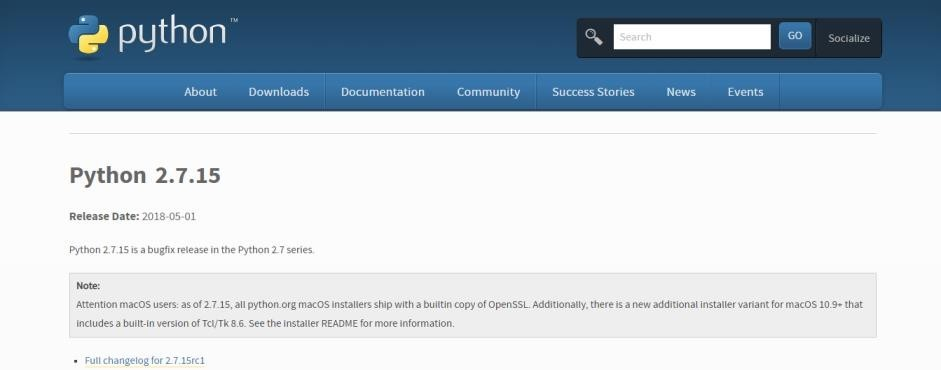
\includegraphics[width=1\textwidth]{figures/8/python.jpg}}
	\caption{Download Softfile Python 2.7.}
	\label{fig:python}
\end{figure}

\item Setelah berhasil mendownload mentahan pythonnya silahkan lakukan instalasi seperti biasa anda lakukan. Setelah selesai instalasi pythonnya silahkan check di Command Prompt, apakah Pythonnya telah terbaca / running disesuaikan dengan laptop anda atau belum. Contoh pengecekan di Command Prompt seperti pada gambar \ref{fig:cek_python27}
\begin{figure}[!htbp]
	\centerline{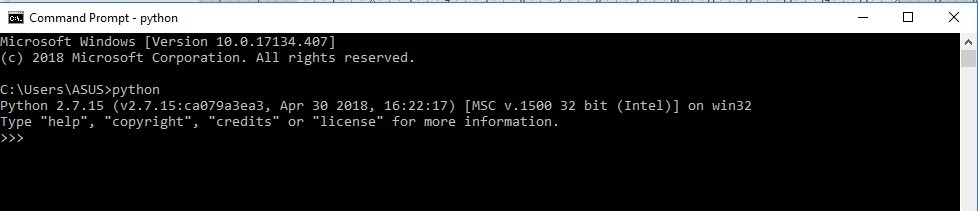
\includegraphics[width=1\textwidth]{figures/8/cek_python27.jpg}}
	\caption{Pengecekan Python 2.7.}
	\label{fig:cek_python27}
\end{figure}

\item Apabila tampilannya telah sesuai dengan gambar \ref{fig:cek_python27}, maka python anda siap digunakan.
\item Pastikan python yang terbaca versi 2.7.15 atau bahkan belum ada sama sekali silahkan lakukan konfigurasi ini:
\begin{itemize}
\item Silahkan buka Control Panel anda.
\item Pilih System and Security.
\item Kemudian pilih lagi system.
\item Lalu  di  bagian  kiri  tampilan  ada  sub menu  Advanced  system setting.
\item Pada  sub  menu  tersebut  silahkan  pilih  button  Environment Variabel.
\item Silahkan ganti path dengan \verb|C:\Python27| dan \verb|C:\Python27\Scripts| ( Lokasi anda menyimpan mentahan python yang telah anda install tadi ).
\item Maka tampilannya akan seperti pada gambar \ref{fig:editenv}.
\begin{figure}[!htbp]
	\centerline{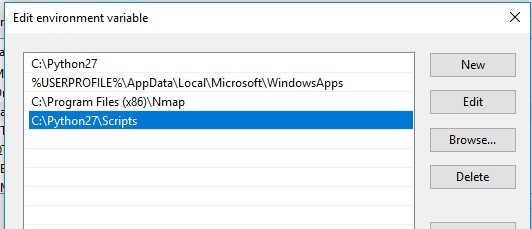
\includegraphics[width=1\textwidth]{figures/8/editenv.jpg}}
	\caption{Pengubahan Environment Python 2.7.}
	\label{fig:editenv}
\end{figure}

\item Jangan lupa untuk memasukkan script dari pythonnya sehingga benar-benar bisa terbaca untuk pipnya. Silahkan klik button ok sampai selesai.
\item Setelah itu, lakukan pengecekan ulang di Command Prompt maka hasilnya akan berubah menjadi versi 2.7.15.
\end{itemize}
\end{enumerate}

\subsection{Instalasi Python 3.6}

Selanjutnya kita mulai dengan tutorial dalam menginstall Python 3.6. Python ini digunakan untuk code pengolahan data csv ke dalam flask python.
\begin{enumerate}
\item Pertama-tama silahkan download software dari python versi 3 di laptop anda. Download python versi 3.6.3 dari situs web resminya yaitu https://www.python.org/. Silahkan sesuaikan dengan kapasitas laptop anda, bisa yang win 32 atau yang win 64 ( 32 bit / 64 bit ). Contoh downloadnya seperti seperti pada gambar \ref{fig:python36}.
\begin{figure}[!htbp]
	\centerline{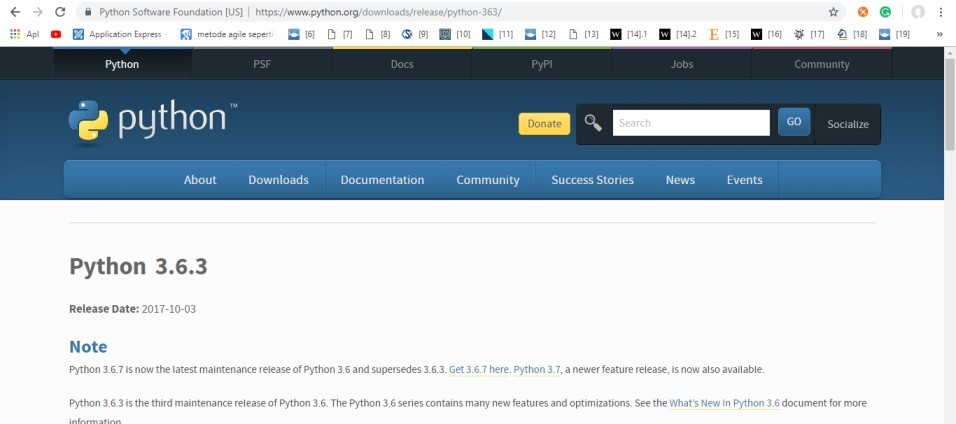
\includegraphics[width=1\textwidth]{figures/8/python36.jpg}}
	\caption{Download Softfile Python 3.6.}
	\label{fig:python36}
\end{figure}
 
\item Setelah berhasil mendownload mentahan pythonnya silahkan lakukan instalasi seperti biasa anda lakukan. Setelah selesai instalasi pythonnya silahkan check di Command Prompt, apakah Pythonnya telah terbaca / running disesuaikan dengan laptop anda atau belum. Contoh pengecekan di Command Prompt seperti pada gambar \ref{fig:cek_python36}
\begin{figure}[!htbp]
	\centerline{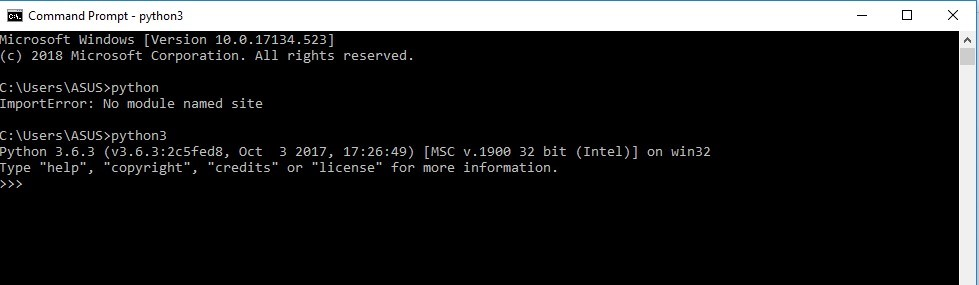
\includegraphics[width=1\textwidth]{figures/8/cek_python36.jpg}}
	\caption{Pengecekan Python 3.6.}
	\label{fig:cek_python36}
\end{figure}

\item Apabila tampilannya telah sesuai dengan contoh diatas, maka python anda siap digunakan.
\item Pastikan python yang terbaca versi 3.6.3 atau bahkan belum ada sama sekali silahkan lakukan konfigurasi ini:
\begin{itemize}
\item Silahkan buka Control Panel anda.
\item Pilih System and Security.
\item Kemudian pilih lagi system.
\item Lalu  di  bagian  kiri  tampilan  ada  sub menu  Advanced  system setting.
\item Pada  sub  menu  tersebut  silahkan  pilih  button  Environment Variabel.
\item Silahkan ganti path dengan \verb|C:\Python27| dan \verb|C:\Python27\Scripts| ( Lokasi anda menyimpan mentahan python yang telah anda install tadi).
\item Maka tampilannya akan seperti pada gambar \ref{fig:editenv36}.
\begin{figure}[!htbp]
	\centerline{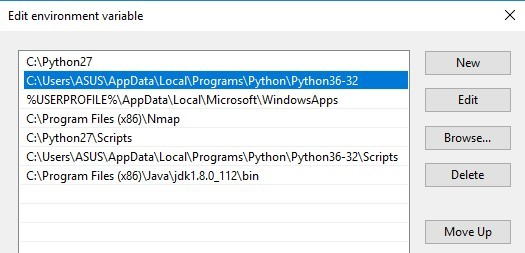
\includegraphics[width=1\textwidth]{figures/8/editenv36.jpg}}
	\caption{Pengubahan Environment Python 3.6.}
	\label{fig:editenv36}
\end{figure}

\item Jangan lupa untuk memasukkan script dari pythonnya sehingga benar-benar bisa terbaca untuk pipnya. Silahkan klik button ok sampai selesai.
\item Setelah itu, lakukan pengecekan ulang di Command Prompt maka hasilnya akan berubah menjadi versi 3.6.3
\item Setelah semua tahap di atas selesai, maka silahkan lanjutkan ke tahap berikutnya.
\end{itemize}
\end{enumerate}

Perintah python flask. Contoh \textit{source code} seperti pada listing \ref{lst:hello}.
\lstinputlisting[caption=Contoh kode program hello.py, label={lst:hello}]{src/8/hello.py}
 Contoh \textit{source code} main.py seperti pada listing \ref{lst:main}.
\lstinputlisting[caption=Contoh kode program main.py, label={lst:main}]{src/8/main.py}
